% ============================================================
% f2013_shanghai_arts_q10_cylinder.tex
% 2013 上海卷（文科）第 10 题 圆柱与异面直线 OA、BC（TikZ 矢量重绘）
% 几何：圆柱母线长 l、底面半径 r；O 为上底面圆心；A、B 在下底面圆周上；
%       BC 为母线（C 在上底面圆周、位于 B 正上方）；直线 OA 与 BC 所成角为 pi/6。
% 说明：示意图，母线方向竖直；底面后半弧画虚线，OA 在柱体内部画虚线。
% ============================================================
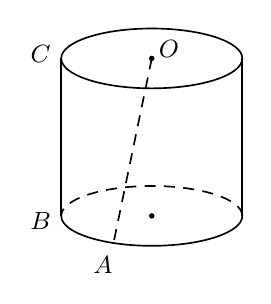
\begin{tikzpicture}[
  x=1cm, y=1cm,
  every node/.style={font=\small, inner sep=1pt},
  line/.style={line width=0.6pt},
  hidden/.style={line width=0.6pt, dash pattern=on 4pt off 3pt},
]

  % 尺寸：底面椭圆半轴、母线长
  \def\rx{1.15}
  \def\ry{0.38}
  \def\hh{2.00}

  % 下底面：前半弧实线，后半弧虚线
  \draw[line] (\rx,0) arc[start angle=0, end angle=-180, x radius=\rx, y radius=\ry];
  \draw[hidden] (\rx,0) arc[start angle=0, end angle=180, x radius=\rx, y radius=\ry];

  % 上底面整椭圆与两条母线轮廓
  \draw[line] (0,\hh) ellipse[x radius=\rx, y radius=\ry];
  \draw[line] (-\rx,0) -- (-\rx,\hh);
  \draw[line] (\rx,0) -- (\rx,\hh);

  % 母线 BC：B 在左端，C 在 B 正上方
  \draw[line] (-\rx,0) -- (-\rx,\hh);

  % 直线 OA（柱体内部，虚线）
  \draw[hidden] (0,\hh) -- (-0.486,-0.344);

  % 上、下底面圆心
  \fill (0,\hh) circle [radius=0.035];
  \fill (0,0) circle [radius=0.035];

  % 标签
  \node at (-\rx-0.26,\hh+0.06) {$C$};
  \node at (0.22,\hh+0.12) {$O$};
  \node at (-\rx-0.26,-0.06) {$B$};
  \node at (-0.62,-0.62) {$A$};

\end{tikzpicture}
